\documentclass[12pt, a4paper]{article}
\usepackage[english, italian]{babel}
\usepackage{enumerate}
\usepackage{babelbib}
\usepackage{verbatim}
\usepackage[utf8]{inputenc}
\usepackage[pdftex]{graphicx}
\usepackage{color}
\usepackage{textcomp}
\usepackage[left=3cm,top=3cm,right=3cm,bottom=3cm]{geometry}
\usepackage{longtable}
\usepackage{listings}

\lstset{
	backgroundcolor=,
	tabsize=4,
	rulecolor=,
	language=Mathematica,
	basicstyle={\scriptsize},
	upquote=true,
	aboveskip={1.5\baselineskip},
	columns=fixed,
        showstringspaces=false,
        extendedchars=true,
        breaklines=true,
        prebreak=% \raisebox{0ex}[0ex][0ex]{\ensuremath{\hookleftarrow}},
		,
        frame=single,
        showtabs=false,
        showspaces=false,
        identifierstyle=\ttfamily,
        keywordstyle=\ttfamily\color[rgb]{0,0,1},
        commentstyle=\ttfamily\color[rgb]{0.133,0.545,0.133},
        stringstyle=\ttfamily\color[rgb]{0.627,0.126,0.941},
}

\title{Relazione sul corso di Metodi Computazionali della Fisica}
\author{Giorgio Ruffa}

\begin{document}

\maketitle

\tableofcontents

\section{Breve introduzione agli Algoritmi Genetici}
\label{sec:intro}
Gli AG sono un particolare tipo di algoritmo che viene utilizzato per risolvere problemi il cui spazio delle soluzioni sia particolarmente vasto. 

Concetto fondamentale degli AG e' considerare un programma come un individuo formato da un'insieme di istruzioni ordinate. questa lista di istruzioni puo' essere assimilata al genoma del nostro individuo e come tale puo' essere modificato. se per esempio prendiamo 2 individui piu' o meno differenti, li tagliamo in due e ne scambiamo le estremita' otterremo 2 nuovi programmi a loro volta eseguibili.
questo meccanismo di taglio e scambio viene detto CrossOver.

Altro concetto centrale e' quello di Fitness. la fitness modellizza quella che e' la capacita' di un individuo reale (quale puo' essere un animale) di adattarsi all'ambiente che lo circonda. dal punto di vista computazionale non e' altro che un voto che viene assegnato all'individuo a seconda della sua capacita' di risolvere un problema. la fitness verra' poi utlizzata per fovorire o meno la riproduzione dell'individuo. individui con la fitness maggiore avranno maggiore possibilita' di riprodursi(Fitness Proportionate). Questo dovrebbe garantire una convergenza verso la soluzione migliore al nostro problema.

possiamo quindi sitetizzare gli step che compongono un AG:

\begin{enumerate}
	\item generazione causale della prima popolazione
	\item valutazione degli individui tramite l'applicazione di una fitness
	\item formazione delle coppie di individui in funzione della fitness
	\item riproduzione degli individui tramite crossover
	\item eventuale mutazione
\end{enumerate}


\section{Problema}
il problema che ci proponiamo di risolvere e' all'apparenza semplice:
immaginiamo di avere un numero di mattoncini su ognuno dei quali sia scritta una lettera e che l'insieme delle lettere formi una parola di senso compiuto (nel nostro caso la parola sara' ``universal'').
le lettere possono o essere inpilate verticalmente formando una stack oppure lasciate sul tavolo.
l'obbiettivo del nostro GA e' di trovare un programma che data una configurazione iniziale delle nostre lettere sia in grado di ricostruire la parola cercata sulla stack.
il programma ha a disposizione un numero limitato di operazione divise in operazioni di lettura , operazioni di movimento, operazioni logiche:

\begin{table}[hbp]
\begin{tabular}[b]{|l|l|}
\hline
\multicolumn{2}{|c|}{lettura} \\
\hline
CS[ ] 	& l'attuale lettera in cima alla stack \\
TB[ ] 	& l'ultimo blocco corretto nella stack \\
NN[ ] 	& la prosiama lettera necessaria a formare la parola\\
\hline
\multicolumn{2}{|c|}{movimento}\\
\hline
MTT[spam]	& se spam e' l'ultima lettera della stack allora mettila sul tavolo\\
MTS[spam]	& metti la lettera spam sulla stack \\
\hline
\multicolumn{2}{|c|}{logica}\\
\hline
DU[work,test]	&	esegui work finche test non diventa vero\\
EQ[expr1,expr2] &	esegui in ordine expr1 ed expr2 e poi controlla se sono uguali\\
NOT[expr] 		&	se expr e' LispNil ritorna vero, altrimenti falso \\
\hline
\end{tabular}
\caption{lista introduttiva delle funzioni}
\label{table:introfun}
\end{table}


un individuo sara' quindi un insieme di istruzioni del tipo
\footnote{per gli aspetti piu' tecnici riguardanti la valutazione dell'individuo, il crossover e i return delle funzioni si veda la sezione \ref{sec:funmoves} }:


\begin{center}
\begin{table}[hbp]
\begin{tabular}[b]{|l|p{7.5cm}|}
\hline
MTT[CS[ ]] & sposta l'ultima lettera della stack sul tavolo\\
DU[MTS[NN[ ]],NOT[NN[ ]]] & sposta la prossima lettera sulla stack finche' non hai terminato la parola cercata.\\
EQ[MTT[CS[ ]] ,MTS[NN[ ]] & prima muovi l'ultima lettera della stack sul tavolo e poi prendi la prossima lettera necessaria del tavolo e mettila sulla stack \\ 
\hline
\end{tabular}
\caption{esempi di individui}
\label{table:esind}
\end{table}
\end{center}

\section{Ambiente di sviluppo e Modellizzazione}
\subsection{Wolfram Mathematica 8}
davanti ad un problema di questo tipo appare di capitale importanza l'utilizzo di strumenti che permettano di manipolare espressioni in maniera facile ed efficiente minimizzando l'implementazione e il debugging. si necessita quindi di un linguaggio per sua natura ad alto livello e con una spiccata flessibilita'.

Per venire incontro a queste esigenze si e' scelto di utilizzare come ambiente di sviluppo {\itshape Wolfram Mathematica 8} \cite{mathematica8} che possiede queste qualita' all'interno del core fondante del linguaggio.

andiamo ad analizzare perche'  {\itshape Mathematica} \cite{mathematica8} si adatta particolarmente bene alle nostre esigenze.
Per quanto possa essere pedante e' bene insistere su concetti di base senza i quali la lettura del package sarebbe particolarmente ostica. Nelle prossime sezioni viene spiegato sinteticamente come {\itshape Mathematica} rappresenti le espressioni e quali comandi possono essere utilizzati per analizzarle e modificarle. Il lettore e' libero di saltarle se possiede gia' buone conoscenze di questi argomenti.

\subsubsection{ogni programma e' un'espressione}
\label{sec:tree}
{\itshape mathematica} tratta ogni statement come un espressione ed ogni espressione ha una struttura ben definita.
prendiamo come riferimento l'ultimo dei nostri programmi d'esempio (si veda tabella ~\ref{table:esind})  .
{\itshape Mathematica} organizza l'espressione sotto forma di albero(figura \ref{figure:estree}).
l'albero e' diviso in livelli ed ogni livello ospita delle sottoespressioni. nel nostro esempio il primo livello contiene le sottoespressioni MTT[CS[ ]] e  MTS[NN[ ]].
mentre il secondo contiene CS[] e NN[]. possiamo ottenere le sottoespressioni contenute in un livello con il comando {\itshape Level[expr,\{livello\}]}. se invece vogliamo l'elenco di tutte le sottoespressioni presenti fino al livello {\itshape n} bastera' dare il comando {\itshape Level[expr,n]}. Nel nostro caso l'output del comando {\itshape Level[individuo,2]} e' \{CS[], MTT[CS[]], NN[], MTS[NN[]]\} infine il comando {\itshape Level[individuo,Infinity]} ci restituisce tutte le possibili sottoespressioni contenute nell'individuo.

ogni espressione (sottoespressioni comprese) possiede una Head, che nel nostro caso non e' altro che il nome della funzione (vengolo elisi i parametri). per esempio la Head del nostro individuo e' EQ e la possiamo ottenere con il comando {\itshape Head[individuo]}.

all'interno della struttura ad albero ogni sottoespressione ha una posizione ben precisa che permette di estrarla e manipolarla facilmente. Per ottenere la posizione di una sottoespressione e' sufficiente utilizzare il comando {\itshape Position[expr,subexpr]} che restituisce un lista di numeri che permette di "risalire" l'albero fino a raggiungere la sottoespressione cercata.

un esempio sara' chiarificatore: {\itshape Position[individuo,CS[]]} resituisce \{2,1\}. Il primo numero ci dice che la nostra sottoespressione e' ``figlia'' del secondo argomento posto al primo livello, mentre il secondo ed ultimo numero ci dice che la sottoespressione e' il primo argomento del nodo ``padre''.

nel caso la sottoespressione appaia piu' di una volta in un espressione {\itshape Position} resitira' una lista di posizioni.

la posizione di una sottoespressione viene utilizzata da comandi come {\itshape Extract} e {\itshape ReplaePart} rispettivamente per estrarre e modificare un sottoespressione mantenendo intatta il resto dell'albero.

\begin{figure}[h]
\begin{center}
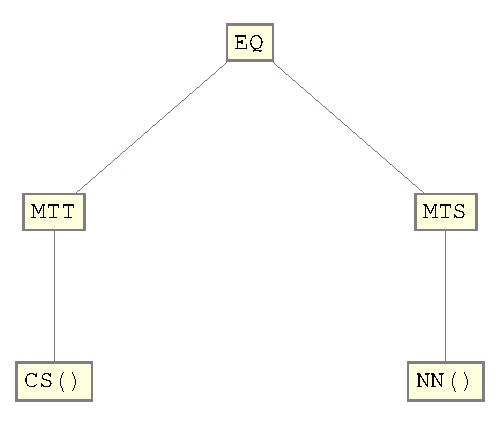
\includegraphics[width=8.0cm]{esempio_albero.pdf}
\caption{struttura ad albero di un espressione (puo' essere ottenuta tramite il comando 
{\itshape TreeForm} )}
\label{figure:estree}
\end{center}
\end{figure}


\subsubsection{Variabili, Funzioni e Parametri}
Un'altra caretteristica importante che garantisce una grande flessibilita' di implementazione e' costituita dalla dinamicita' delle assegnazioni. Essendo essenzialmente un linguaggio non tipizzato e ad alto livello (davvero molto alto) al nome di una variabile puo' corrispondere qualsiasi valore di un espressione e questo valore puo' venire cambiato in qualsiasi punto del codice senza doversi preoccupare dell'allocazione di memoria e di name-lookup. Questa caratteristica torna particolarmente comoda quando si devono introdurre nuove variabili come per esempio parametri per il calcolo della fitness, liste per la registrazione dei trend delle caratteristiche delle popolazioni, oppure strumenti per l'analisi e la visualizzazione dei dati raccolti. In un linguaggio tipizzato questo avrebbe richiesto un massiccio intervento sulla struttura del codice, soprattutto nel caso di linguaggi Object Oriented (dove si puo' essere costretti a ridisegnare grandi sezioni della struttura di ereditarieta')

In questo quadro e' bene introdurre le variabili principali utilizzate nel package:
la stack e il tavolo (da ora in avanti espresse anche come Table e Stack) sono 2 liste che possono essere modificate solo dalle funzioni MTT e MTS.
la parola di riferimento (TargetWord) e' uguale a \{l,a,s,e,r,v,i,n,u\}; il fatto che la disposizione delle lettere sia al contrario e' semplicemente perche' la Stack viene letta dall'alto verso il basso e la prima lettera e' quella a contatto con il tavolo, in questo modo l'implementazione risulta di molto semplificata.

la fitness sara' una funzione che esaminera' la stack formata dall'individuo per confrontarla con la parola finale ed eventualmente potra' considerare anche altre caratteristiche dell'individuo, come per esempio l'efficienza e il numero di operazioni che esegue.


\section{I Moduli}
dopo aver ben chiaro come {\itshape Mathematica} struttura e interfaccia le espressioni possimo passare ad una analisi dei moduli che compongono il package.
in questa sezione troverete esplicate le principali funzioni utilizzate divise in cinque moduli e accompagnate dalle parti piu' significative del codice con commenti annessi
\footnote{in appendice e' riportato l'intero codice}.

\subsection{Le funzioni di base}
Vengono riportate in questo file tutte le operazioni che gli individui possono effettuare, il loro nome esteso, la descrizione , i return ed eventualmente inclusioni di codice significativo. 
Le funzioni qui' documentate si trovano nel file {\itshape moves.m}
\subsubsection{Variabili}
\label{sec:varmoves}
la variabili presenti nel file hanno lo scopo di renderlo indipendente dagli altri moduli. cosi' facendo il modulo puo' essere testato separatamente.
\begin{description}
	\item{TargetWord:} \{l,a,s,r,e,v,i,n,u\} la parola che cerchiamo di ricostruire 
	\item{MyStack:} la stack, e' una lista.
	\item{MyTable:} il tavolo, e' una lista.
	\item{maxdustep:} numero massimo di esecuzioni di {\itshape work} dopo le quali il DU non viene piu' valutato e viene considerato Broken.
	\item{BrokenDU:} numero di DU broken.
	\item{StepCount:} numero di step, gli step di un individuo sono il numero di volte che una lettera viene spostata.
	\item{LispNil:} per garantire la conformita' con la letteratura\cite{mitchell} e una facilita' di gestione dei processi alcune funzioni possono ritornare questa variabile che al momento e' settata ad una stringa.
\end{description}

\lstset{caption=variabili di moves.m,
		label=source:movesvar}
\lstinputlisting{moves_var.m}

\subsubsection{Funzioni}
\label{sec:funmoves}

\begin{longtable}{|l|p{10.0cm}|}
%\begin{tabular}{|l|p{10.0cm}|}
\hline
funzione:		& 	CS[ ]\\
nome esteso:	& 	current stack\\
comportamento:	& 	restituisce l'ultima lettera della stack,se la stack e' vuota ritorna LispNil\\
return:			& 	una lettera o LispNil\\
\hline
\multicolumn{2}{|c|}{}\\

\hline
funzione:		& 	TB[ ]	\\
nome esteso:	& 	top correct block\\
comportamento:	& 	ritorna l'ultima lettera che si trova in posizione corretta sulla stack. se nessuna lettera e' in posizione corretta ritorna LispNil\\
esempio:		&	MyStack = \{l,a,n,i\} ; In:TB[ ] ; Out: a \\
return:			& 	una lettera o LispNil\\
\hline
\multicolumn{2}{|c|}{}\\

\hline
funzione:		& 	NN[ ]\\
nome esteso:	& 	next needed\\
comportamento:	& 	ritorna la prossima lettera necessaria per formare la TargetWord. se la stack forma gia' la TargetWord ritorna LispNil\\
return:			& 	una lettera o LispNil\\
\hline
\multicolumn{2}{|c|}{}\\

\hline
funzione:		& 	MTS[{\itshape spam}]\\
nome esteso:	& 	move to the stack\\
comportamento:	& 	prendi la lettera {\itshape spam} dal tavolo e la mette in cima alla stack (la mette come ultima lettera della lista MyStack) e ritorna la lettera spostata. se la lettera non e' sul tavolo non fa niente e ritorna comunque la lettera {\itshape spam}.\\
return:			& 	sempre una lettera\\
\hline
\multicolumn{2}{|c|}{}\\

\hline
funzione:		& 	MTT[{\itshape spam}]\\
nome esteso:	& 	move to the table\\
comportamento:	& 	se la lettera {\itshape spam} e' in cima alla stack (e' l'ultima lettera di MyStack) spostala sul tavolo e ritorna {\itshape spam}. se {\itshape spam} non e' in cima alla stack non fare niente e ritorna {\itshape spam} \\
return:			& 	sempre una lettera\\
\hline
\multicolumn{2}{|c|}{}\\

\hline
funzione:		& 	NOT[{\itshape expr}]\\
nome esteso:	& 	not\\
comportamento:	& 	se expr e' LispNil ritorna True, in tutti gli altri casi ritorna False\\
return:			& 	True o False\\
\hline
\multicolumn{2}{|c|}{}\\

\hline
funzione:		& 	EQ[{\itshape expr1 , expr2}]\\
nome esteso:	& 	equal\\
comportamento:	& 	valuta prima expr1, poi expr2 e ritorna True se i risultati sono uguali, altrimenti ritorna false\\
return:			& 	True o False\\
\hline
\multicolumn{2}{|c|}{}\\

\hline
funzione:		& 	DU[{\itshape work , test}]\\
nome esteso:	& 	do untill\\
comportamento:	& 	valuta work finche' test non restituisce True. Ritorna LispNil se work viene eseguido piu' volte di {\itshape maxdustep}, altrimenti Null\\
return:			& 	Null o LispNil\\
\hline
%\end{tabular}
\caption{operazioni che un individuo puo' fare}
\label{table:basicfun}
\end{longtable}

\lstset{caption=implementazione delle funzioni di base,
		label=source:basfun}
\lstinputlisting{moves_insert.m}

\begin{comment}
(************************************************************)
\hline
funzione:		& 	\\
nome esteso:	& 	\\
comportamento:	& 	\\
return:			& 	\\
\hline
(************************************************************)
\end{comment}


\subsubsection{Note Tecniche}
la funzione DU altro non e' che un contenitore (wrapper) per un While e come si puo' vedere ha settato come attributo {\itshape HoldAll}. la necessita' di utilizzarlo nasce dal fatto che quando viene chiamata una funzione {\itshape Mathematica} valuta subito i suoi argomenti e assegna il risultato della valutazione ad ogni ricorrenza del nome della variabile nel codice della funzione e successivamente la esegue. in questo modo se l'espressione {\itshape test} e' False la prima volta che viene chiamato il DU, continuera' ad esserlo a prescindere dall'azione che Work fa sulla Stack e sul tavolo. Questo puo' portare a comportamenti anomali e loop infiniti. L'attributo {\itshape HoldAll} forza {\itshape Mathematica} a non valutare gli argomenti delle funzioni quando vengono chiamate, in questo modo le espressioni vengono valutate in runtime durante l'esecuzione della funzione.
\footnote{l'utilizzo di HoldAll e' stato particolarmente istruttivo permettendomi di comprendere meglio meglio come Mathematica gestisca la chiamata delle funzioni.}


\subsection{Generazione degli Individui}
questa sezione analizza il contenuto del file {\itshape firstgen.m} che contiene
il primo step di ogni algoritmo genetico: la generazione di una prima popolazione di individui.

\subsubsection{correttezza sintattica}
\label{sec:sintax}
Normalmente la generazione viene fatta casualmente ma in questo particolare caso e' stato scelto di formare individui che siano sempre sintatticamente corretti. ovvero costrutti del tipo  CS[MTT[ ]] che non hanno alcun senso dal punto di vista sintattico non devono essere presenti.

Il modo in cui ho affrontato il problema e' il seguente: presa una delle 8 funzioni (vedi tabella \ref{table:basicfun} a pag \pageref{table:basicfun}) essa potra' avere solo un numero limitato di argomenti possibili. Per esempio MTT potra' avere come argomento solo quelle funzioni che restituiscono una lettera, altrimenti la funzione non e' definita e non verra' eseguita da Mathematica;

per poter guadagnare in flessibilita' ho scelto di utilizzare delle liste di argomenti permessi. Ad ogni funzione e' associata una lista dalla quale verra' estratta una funzione corretta. In questo modo posso cambiare in qualsiasi momento le regole sintattiche e questo e' un vantaggio da non sottovalutare.

in seguito e' allegata l'implementazione:

\lstset{caption=liste compatibilita',
		label=source:complist}
\lstinputlisting{complist.m}

come si puo' notare per il DU appaioni due liste: DUW e DUT , che stanno rispettivamente per DUWork e DUTest. essenzialmente il primo e il secondo argomento di DU differiscono per regole sintattiche, il {\itshape test} dovra' essere una funzione che restituisce o True o False mentre il {\itshape Work} puo' essere qualsiasi funzione.

la presenza di variabili in caratteri minuscoli (come {\itshape e1,e2,n, \ldots}), viene spiegata nella sezione \ref{sec:generic}.

\subsubsection{valutazione ritardata}
come si vede nel listato \ref{source:complist} le funzioni appiono con una {\itshape f} come prima lettera. Se non ci fosse questa lettera le funzioni verrebbero valutate subito ad ogni loro ricorrenza nel codice, metre l'obbiettivo e' di valutarle tramite la chiamata di funzioni apposite che effettueranno la sostituzione con le funzioni vere e proprie. Per quanto possa sembrare artificiosi in realta' si sta' semplicemento dando un nome diverso alle funzioni, un nome che non ha alcuna definizione implementata. \footnote{per maggiori informazioni si veda la sezione \ref{sec:valmec} a pagina \pageref{sec:valmec}}

\subsubsection{generazione ricorsiva}
\label{sec:generic}
Per sfruttare al meglio la struttura ad albero esposta nella sezione \ref{sec:tree} ho deciso di generare gli individui con un algoritmo ricorsivo che percorra tutti i ``rami'' dell'albero.
In sostanza l'algoritmo consiste nel generare una prima Head a caso dalla lista EQList\footnote{EQList contiene tutte le funzioni} e poi chiamare una funzione che data la head del ``padre''  e' in grado di scegliere un argomento a caso dalla lista di compatibilita' del padre e richiamare se stessa sugli argomenti ``figli''.

La funzione che implementa questo algoritmo e' {\itshape HAC} \footnote{Head A Caso} (si veda listato \ref{source:HAC}).

La prima definizione viene usata la prima volta. Chiamando il comando {\itshape HAC[]} la funzione sceglie una Head random che sara' per esempio {\itshape fEQ[e1,e2]}, a questo punto appare ovvia l'importanza delle variabili {\itshape e1 e2} menzionate in \ref{sec:sintax}: tramite la lista di sostituzioni chiamata {\itshape sostituzioni} mi permettono di chiamare la funzione {\itshape HAC[fathhead\_]} con la Head del ``padre'' corretta. Dopo la prima chiamata di HAC abbiamo un espressione del tipo fEQ[ HAC[fEQ1] , HAC[fEQ2] ]. 

A questo punto viene eseguita la seconda funzione del listato (per esempio HAC[fEQ1]), che sceglie a sua volta un argomento che puo' stare a primo membro di fEQ e richiama se stessa sugli argomenti ottenuti in modo analogo a come descritto prima. la scelta dell'argomento viene effettuata con la funzione ChooseArg (il codile e' nella sezione \ref{sec:source}).

Come in ogni algoritmo ricorsivo sono necessarie delle condizioni di uscita senza delle quali la generazione si arresterebbe nel caso in cui tutte le chiamate residue di {\itshape HAC[fathhead\_]} resituissero NN[] CS[] o TB[]. Questo potrebbe portare ad una generazione iniziale di individui troppo complessi per i nostri scopi, di conseguenza viene messo un limite al numero di volte che HAC viene chiamato per singolo individuo e al numero di foglie che l'individuo possiede \footnote{si veda comando LeafCount}.
E' la funzione {\itshape RigthInd[]} che genera un individuo sempre corretto premurandosi di controllare anche che il numero di foglie non superi un certo limite.
La definizione di questi limiti a livello di implementazione e' trattata nella sezione seguente.

\subsubsection{variabili}
all'interno del file firstgen.m sono presenti le seguenti variabili:
\begin{description}
	\item{Nind : } numero di individui che compongono la prima generazione (utilizzata per testare il singolo file);
	\item{MaxHacCall : } numero massimo di chiamate di HAC oltre le quali la generazione dell'individuo si arresta;
	\item{CurrHacCall : } attuale numero di chiamate di HAC (utilizzata per testare il singolo file);
	\item{MinLeaf : } numero minimo di foglie che un individuo deve avere;
	\item{ManLeaf : } numero massimo di foglie che un individuo deve avere;
\end{description}

\lstset{caption=la funzione HAC per la generazione ricorsiva degli individui,
		label=source:HAC}
\lstinputlisting{hac_insert.m}


\subsection{Meccanismo di Valutazione}
\label{sec:valmec}
La valutazione di un individuo e' una parte fondamentale in quanto ricorre Nind volte per generazione. Non deve solo valutare l'individuo ma generare dei dati che verranno passati alla fitness per valutare quanto l'individuo si sia comportato correttamente. Infine deve essere molto semplice da utilizzare, deve quindi avere un'interfaccia pulita. Con Mathematica tutto questo puo' essere fatto in una trentina di righe di codice in una singola funzione, come possiamo vedere dal listato \ref{source:EvalInd}.

La funzione {\itshape EvalInd[ind\_]} valuta un individuo e restituisce la Stack ottenuta alla fine della valutazione, il numero di BrokenDU occorsi, il numero di Step eseguiti
\footnote{ per il significato di queste variabili si veda \ref{sec:varmoves}}
, e la Richness dell'individuo.
\footnote{la richness e' spiegata nella sezione \ref{sec:fit}}

La funzione {\itshape Block} forza le variabili contenute nella lista ad avere il valore che gli viene assegnato localmente, in questo modo per ogni individuo la Stack e la Table vengono riportate alla configurazione iniziale e poi restituite dalla funzione per essere analizzate dalla fitness.

\lstset{caption=funzione che valuta un individuo , label=source:EvalInd}
\lstinputlisting{val.m}



\subsection{Crossover}
il crossover e' la parte che piu' caratterizza un algoritmo genertico e in questo Package e' una delle fasi tecnicamente piu' complesse.
esso deve mantenere la correttezza sintattica degli individui e garanetire che lo scambio venga eseguito sempre (qualora la correttezza sintattica lo permettesse).

questa sezione analizza la funzione {\itshape CrossOver} presente nel file {\itshape crossover.m}.

\subsubsection{garantire la correttezza sintattica}
In sommi capi il CrossOver deve tagliare due individui in due parti e scambiarle. Se in generale questa e' un operazione semplice, nel nostro caso il fatto di dover garantire la correttezza sintattica complica le cose. 

Chiariamo cosa si intenda per ``punto di taglio'': ogni sottoespressione\footnote{si veda sezione \ref{sec:tree}} presente in un individuo sara' un argomento di una delle otto funzioni fondamentali e, se l'individuo e' stato generato correttamente, sara' nella sua lista di compatibilita'.
\footnote{si veda listato \ref{source:complist} pagina \pageref{source:complist}} 

un punto di taglio sara' quindi una coppia costituita da una sottoespressione e dalla Head della funzione di cui la sottoespressione e' argomento.

per comodita' la sottoespressione del primo individuo sara' chiamata ``Ramo1'' e la funzione di cui Ramo1 e' argomento la chiameromo HeadPadre1.
Ramo2 sara' analogamente la sottoespressione del secondo individuo , e HeadPadre2 la funzione di cui Ramo2 e' argomento.
\footnote{TODO: ESEMPI CON FIGURE}

Per garantire la correttezza sintattica dovranno essere presenti contemporaneamente due condizioni:
Ramo2 deve essere compatibile con HeadPadre1 e Ramo1 dovra' essere compatibile con HeadPadre2.
bisognera' quindi scegliere una coppia di punti di taglio che permetta il CrossOver.

\subsubsection{garantire lo scambio}
Ad un primo tentativo il crossover puo' non trovare una coppia di punti di taglio corretti. Nelle prime generazioni questo fenomeno non e' trascurabile e porta a delle modificazioni sensibili della probabilita' di CrossOver. Per ovviare a questa situazione l'algoritmo dovra' cercare di considerare tutti i punti di taglio possibili finche' non trovera' una coppia adatta.

\subsubsection{l'algoritmo}
La funzione CrossOver[] opera i seguenti passaggi:
\begin{enumerate}
\item genera una lista di tutte le sottoespressioni dellindividuo 1 e la mescola in maniera random;
\item partendo dalla prima genera una lista di Ramo2 compatibili con HeadPadre1, che chiameremo ``Candidati''.
\item riordina Candidati casualmente
\item passa in sequenza i membri di Candidati finche' HeadPadre2 non e' compatibile con Ramo1
\item se hai trovato una buona coppia di punti di taglio effettua lo scambio, altrimenti restituisci gli individui intatti ed incrementa un contatore.
\end{enumerate}

questa procedura ha permesso di minimizzare i casi di fallimento del crossover nelle prime generazioni da circa 10/100 a circa 1/100.\footnote{test effettuati su popolazioni di 200 individui alla prima generazione}

\subsubsection{variabili}
le due variabili presenti nel file sono PartialCrossFail , TotalCrossFail. la prima viene utilizzata per conteggiare quanti crossover falliscono perche' l'individuo 1 non ha candidati compatibili per il taglio, mentre il secondo conteggia i crossover falliti perche' nessuna HeadPadre2 dei candidati e' compatibile con nessun Ramo1.

\subsubsection{note tecnice}
data la lunghezza l'algoritmo e' riportato bella sezione \ref{sec:source}.
Le funzioni di {\itshape Mathematica} fondamentali in questo algoritmo sono: 
\begin{itemize}
\item il comando Positon[ind,subexpr] gia' menzionato nella sezione \ref{sec:tree}; 
\item il comando Extract[ind,position] che restituisce la sottoespressione che si trova nella posizione {\itshape position} dell'individuo {\itshape ind}
\item il comando ReplacePart[ind,position \verb|->| expr] che permette di sostituire all'interno dell'individuo la sottoespressione che si trova in {\itshape position} con l'espressione {\itshape expr}
\item il comando RandomSample[list] che riordina casualmente una lista {\itshape list}
\item il comando RandomChoice[list] che restituice un elemento random della lista {\itshape list}
\end{itemize}

si consiglia la retturna della reference per le funzioni sopracitate. 

\subsubsection{considerazioni}
il CrossOver in questo caso non conserva la lunghezza degli individui che tenderanno ad aumentare per profondita' e complessita' con l'andare delle generazioni.
\footnote{si veda \ref{sec:exp}}


\subsection{Fitness}
\label{sec:fit}
La Fitness e' sicuramente la parte decisiva nel succeso di un algoritmo genetico e modellizzando quello che e' l'ambiente per gli esseri viventi.

La scelta fatta nello scrivere la Fitness e' stata di garantire una certa modularita'.

La modellizzazione e' la seguente: ogni caratteristica di un induviudo viene valutata con un punteggio.
ogni punteggio ha un peso e la somma dei punteggi pesati costituisce il voto finale dell'individuo.

le caratteristiche valutate sono:
\begin{table}[h]
\begin{tabular}{|l|p{10.0cm}|}
\hline	\\
RigthLetters	&	un punto per ogni lettera implata correttamente sulla stack	\\
DidSome			&	un punto per ogni lettera che differisce dalla stack iniziale piu' un punto per ogni differenza di dimensione tra stack iniziale e finale	\\
Richness		&	un punto per ogni ognuna delle otto funzioni base presente nell'individuo	\\
BrokenDU		&	un punto per ogni BrokenDU	\\
Step			&	un punto per ogni step fatto	\\
\hline
\end{tabular}
\caption{aspetti valutati dalla fitness}
\label{table:fitfunc}
\end{table}

I punteggi ci danno una sorta di fotografia comportamentale dell'individuo, ma la vera selettivita' consiste nel peso che viene affidato ad ogni singolo punteggio.
Possiamo decidere di premiare individui particolarmente attivi o ricchi di funzioni base, oppure possiamo premiare individui che fanno un numero di step prestabilito o un numero di BrokenDu piccolo.

Per esempi e risposta della popolazione a particolari tipi di selezione si veda la sezione\ref{sec:exp}

\subsubsection{implementazione}
La fitness e' una funzione che si applica al singolo individuo e che per le sopracitate scelte di modularita' e' stata divisa in step diversi.
\begin{enumerate}
\item la valutazione degli individui produce una lista di risultati descritta in \ref{sec:valmec} a pagina \pageref{sec:valmec}
\item il risultato della valutazione viene passato alla funzione FitnessParameters che si occupa di applicare le funzione di valutazione in tabella \ref{table:fitfunc} e di resituire i punteggi in modo ordinato.
\footnote{i BrokenDu e gli Step vengono calcolati nel momento della valutazione dell'individuo, nessuna funzione viene appliacata di FitnessParameters ma vengono semplicementi copiati all'interno della lista dei risultati}
\item infine i punteggi calcolati da FitnessParameters vengo dati in pasto alla funzione Fitness che li elabora secondo i pesi scelti ed eventali altri aspetti
\end{enumerate}

il vantaggio di questa procedura consiste nel poter raccogliere piu' facilmente le valutazioni degli individui per costruire strumenti diagnosctici con estrema flessibilita'.
\footnote{si veda sezione \ref{sec:tools} }

\subsubsection{considerazioni}
E' stato scelto di non dare punteggi negativi ma premiare di meno individui che non hanno certe caratteristiche. In questo modo e' possibile registrare un trend della fitness media ed avere quindi un punto di riferimento sulla convergenza della popolazione.

Ho scelto di non valutare caratteristiche "fisiche" degli individui, come per esempio il numero di foglie o la profondita'\footnote{si vedano comandi LeafCount e Depth}, ma di valutare il solo comportamento degli individui, questo non ha comunque precluso la possibilita' di trovare risultati significativi.

\subsection{Tools}
\label{sec:tools}
la parte finale dell'implementazione e' stata dedicata a costrure degli strumenti che permettessero di analizzare velocemente e in maniera semplice le caratteristiche di una generazione e del suo sviluppo al passare delle iterazioni dell'algoritmo.

Anche in questo caso {\itshape Mathematica} ha offerto un insieme di strumenti che hanno reso snella l'implementazione.

Per permettere questo genere di analisi le caratteristiche, come per esempio le singole stack degli individui alla fine della valutazione o le singole fitness, vengono salvate in apposite liste che vengono riempite dalla funzione Profiler che si trova nel file {\itshape fitness.m}, per poi essere lette dalle funzioni presenti in {\itshape tools.m}.

Ecco l'elenco delle funzioni e il loro risultato:
\begin{description}
\item{GenGraphs[n\_]: } stampa una griglia di quattro grafici rappresentanti la fitness, la distribuzione della fitness, il numero di foglie di ogni individuo e la profondita' di ogni individuo;
\item{PlotTrends[]: } stampa una griglia di quattro grafici rappresentanti i valori che le seguenti grandezze hanno assunto nelle generazioni precedenti: fitness media, devianzione standard della fitness , foglie medie e profondita' media.
\item{popgiusti[]: } resituisce una lista di coppie \{numero generazione , numero individui giusti\}, dove per individui giusti si intende quelli che formano la TargetWord a prescindere dalle prestazioni.
\item{perfetti[]: } resituisce una lista di coppie \{numero generazione , numero individui perfetti\}, dove per individui perfetti si intendono quegli individui uguali all'individuo perfetto presente in letteratura;
\footnote{si veda \ref{sec:exp}}
\item{PR[]: } fai un profilo della simulazione effettuata, stampando l'output di popgiust[], i paramentri usati nella simulazione e il numero di generazioni.
\item{ProfileRun[filename\_]: } stampa su file l'output di popgiusti[] , perfetti[], PlotTrends[], i parametri usati e il numero di generazioni.
\item{salvaindividuo[ind\_,filename\_]: } salva l'individuo su un file.
\item{F2D[list\_]: } data una lista restituisce una lista di coppie \{valore, numero di ricorrenze di valore in list\}
\item{ProfileGeneration[n\_]: } data la generazione n salva gli individui che formano la TargetWord nella variabile {\itshape giusti} e il prodotto delle loro valutazioni in {\itshape valgiusti}
\end{description}

un uso approfondito di questi strumenti e' stato fatto nella sezione \ref{sec:exp}

\section{Utilizzo del Package}
in questa sezione troverete come utilizare il Package per generare una popolazione, farla evolvere e analizzare il risultato.

come prima cosa occorre generare una popolazione, settiamo quindi il numero di individui e generiamo la prima popolazione:
\begin{lstlisting}
PM = 0.001;
PC = 0.7;
Nind = 100;
pop = FirstGeneration[];
\end{lstlisting}

ora abbiamo la nostra popolazione di individui formata. Per analizzarla preliminarmente bastera' dare il comando
\lstset{caption=,label=}
\begin{lstlisting}
ListPlot[ F2D[ Map[LeafCount,pop] ] ];
\end{lstlisting}

ottenedo come output qualcosa di simile alla figura \ref{figure:leafcount}

\begin{figure}[!h]
\begin{center}
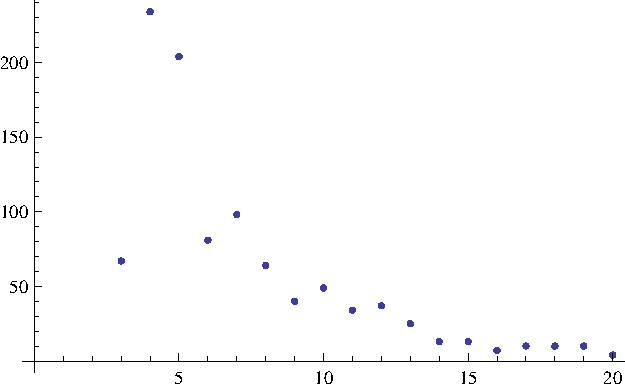
\includegraphics[width=10.0cm]{leafcountlistplot.pdf}
\caption{numero di individui con x foglie}
\label{figure:leafcount}
\end{center}
\end{figure}

ora possiamo fare evolvere la nostra popolazione di uno step con il comando
\begin{lstlisting}
pop2 = StepGen[pop]
\end{lstlisting}
la funzione StepGen[popolazione] esegue tutti i passi di un algoritmo genetico esposti a pag \pageref{sec:intro}, meno che la mutazione e restituisce la popolazione elaborata.

volendo far eseguire piu' generazioni una routine di questo tipo permettera' anche di salvare ogni generazione:
\begin{lstlisting}
gennumebr = 20;
pops = {pop,pop2}
prova[]:= For[incr=3,incr<gennumber,incr++,
				Print["GEN: " , incr];
				gens = 	Append[	pops,
								StepGen[ pops [[incr-1]] 
								] 
						]
];
\end{lstlisting}

infine potremo avere un analisi di insieme della nostra popolazione con il comando PR[] e salvare i risultati con il comando ProfileRun[filenale\_]:
\begin{lstlisting}
PR[]
ProfileRun["rundiprova.m"]
\end{lstlisting}

se siete nel notebook otterrete un output del tipo (figura \ref{figure:tryout}):
\begin{lstlisting}
popolazione totale:
1000
parametri:
{rlw,dsw,riw,bdw,stw,msl,dsl,mdl,ddl}
{250, 1, 5, 500, 1000, 0, 2, 13, 5}
popolazione di elementi perfetti: 
{}
popolazione di elementi giusti: 
{{5, 1}, {18, 1}, {27, 1}, {28, 1}, {29, 2}, {30, 1}, {31, 2}, {32, 1}, 
 {35, 1}}
numero runs:
40
MAXDU:
5
MAXSTEP:
30
\end{lstlisting}

\begin{figure}[!h]
\begin{center}
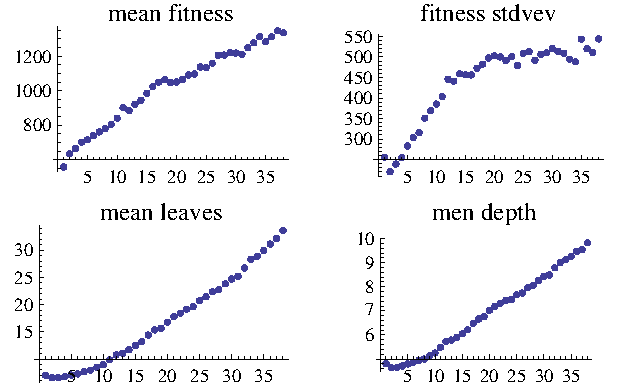
\includegraphics[width=10.0cm]{pr.pdf}
\label{figure:tryout}
\end{center}
\end{figure}

per conoscere meglio come utilizzare il Package si consiglia una lettura della sezione seguente.



%%%%%%%%%%%%%%%%%%%%%%%%%%%%%%%%%%%%%%%%%%%%%%%%%%%%%%%%%%%%%%%%%%%%%%%%%%%%%%%%%%%%%%%%%%%%%%%%%%%%%%%%%%%%%%%%%%%%%%%%%%%%
%%%%%%%%%%%%%%%%%%%%%%%%%%%%%%%%%%%%%%%%%%%%%%%%%%%%%%%%%%%%%%%%%%%%%%%%%%%%%%%%%%%%%%%%%%%%%%%%%%%%%%%%%%%%%%%%%%%%%%%%%%%%
%%%%%%%%%%%%%%%%%%%%%%%%%%%%%%%%%%%%%%%%%%%%%%%%%%%%%%%%%%%%%%%%%%%%%%%%%%%%%%%%%%%%%%%%%%%%%%%%%%%%%%%%%%%%%%%%%%%%%%%%%%%%


\section{Testing e Applicazioni}
\label{sec:exp}
questa sezione vuole rappresentare una scpecie di ``quaderno di laboratorio'' che ha portato ad individuare l'effetto di determinati set di paramentri e regole di selezione sulla qualita' degli individui.
Per idee su possibili sviluppi e miglioramente si veda la sezione \ref{sec:opti}

\subsection{l'individuo perfetto}
come viene indicato in letteratura \cite{mitchell}, esiste la soluzione perfetta al nostro problema, cioe' un individuo che ricostrutisce la parala cercata nel minor numero possibile di mosse.
\begin{table}[h]
\begin{tabular}{|c|}
\hline
EQ[ DU[MTT[CS[]] ,NOT[CS[]]  ] ,DU[MTS[NN[]] , NOT[NN[]] ]  ]\\
\hline
\end{tabular}
\caption{l'individuo ``perfetto''}
\label{table:perf}
\end{table}

come possiamo vedere il primo argomento di EQ e' un DU che svuota completamente la stack, mentre il secondo la riempie con le lettere in ordine corretto.

Le caratteristiche di questo individuo sono le seguenti:
\begin{itemize}
\item un numero di foglie pari a 11
\item una profondita' pari a 5
\item un numero di step pari a 13
\item nessun broken du
\label{item:perf}
\end{itemize}

La ricerca della giusta combinazione di parametri che permettessero a questo individuo di apparire e di riprodursi con successo e' stata la parte finale dell'esperienza di laboratorio.
Questo ha portato allo sviluppo di molti dei tools esposti nella sezione \ref{sec:tools}

\subsection{Condizioni Iniziali}
Per condizioni iniziale si intende la composizione iniziale di Stack e Table. Non solo e' essenziale che tutti gli individui partano dalla stessa configurazione, ma anche che sia identica per tutte le simulazioni. in questo modo il successo di determinati set di parametri non e' riconduciblie a configuarazione particolarmente fortunate della Stack.

Di conseguenza la funzione di valutazione (si veda \ref{sec:valmec}) utilizza due variabili, DefaultStack e DefaultTable, che rappresentano rispettivamnte il valore iniziale della Stack e del Tavolo.

Il valore scelto per queste simulazioni e' stato: 

\begin{lstlisting}
DefaultStack = {u,n,i,v} ;
DefaultTable = {e,r,s,a,l};
\end{lstlisting}

si ricordi che la stack corretta non e' \{u,n,i,v,e,r,s,a,l\}, ma \{l,a,s,e,r,v,i,n,u\};

\subsection{Parametri e funzione Lol}
per parametri si intendono i pesi che vengono dati ai punteggi indicaticati nella sezione \ref{sec:fit} , che sono presenti nella funzione {\itshape Fitness}.
Si veda il listato sottostante.
\begin{lstlisting}
	rlw	=	1000;	(*right letter weight*)
	dsw	=	1;		(*do something weight*)
	riw	=	5;		(*richness weight*) 
	bdw	=	10;		(*broken DU weight*) 
	stw	=	10;		(*step weight*) 
\end{lstlisting}

Inoltre e' stata sviluppata anche una funzione chiamata {\itshape Lol[media\_ , sigma\_ , x\_]} (presente in tools.m) , che data una gaussiana centrata su {\itshape media} e sigma uguale a {\itshape sigma} il cui valore massimo vale 1 restituisce il valore della funzione in {\itshape x}.

essa e' stata utilizzata per premiare quegli individui che avevano un valore di Step piu' o meno vicino ad un valore medio, e un valore di BrokenDU vicino a zero.
infatti, qualora venga fatto l'utilizzo di {\itshape Lol} nella funzione {\itshape fitness}, troverete anche le seguenti variabili:
\begin{lstlisting}
	msl = 13;	(*mean step lol*) 
	dsl = 5;	(*delta step lol*) 
	mdl = 0;	(*mean broken du lol*) 
	ddl = 2;	(*delta broken du lol*) 
\end{lstlisting}

la funzione {\itshape lol} restituisce sempre un valore tra 0 e 1, quindi modula il punteggio dato dai pesi bdw e stw.

\subsection{Primi test sui parametri}
la parte iniziale dell'esprerienza e' stata dedicata a primi test indicativi sull'effetto dei parametri.
\subsubsection{individui giusti}
Chiaramente l'aspetto che piu' mi premeva testare era se l'algoritmo fosse stato in grado di produrre una popolazione di individidui che formassero la TargetWord.
Per fare cio' ho scelto una fitness che premiasse soprattutto gli individui in grado di formare sequenze di lettere in ordine corretto.
Di conseguenza ho usato un valore di {\itshape rlw} particolarmente alto e non ho utilizzato la funzione {\itshape Lol}.

Ecco i risultati della simulazione cosi' come vengono riportati dall funzione {\itshape ProfileRun[filename\_]} (\ref{sec:tools} a pag \pageref{sec:tools}).
\begin{lstlisting}
popolazione totale:
300
parametri:
{rlw,dsw,riw,bdw,stw}
{1000, 1, 5, 10, 10 }
popolazione di elementi perfetti: 
{}
popolazione di elementi giusti: 
{{2, 1}, {3, 13}, {4, 72}, {5, 151}, {6, 211}, {7, 201}, {8, 221}, {9, 228}, 
 {10, 229}, {11, 239}, {12, 249}, {13, 237}, {14, 233}, {15, 248}, {16, 264}, 
 {17, 265}, {18, 264}, {19, 261}, {20, 261}, {21, 274}, {22, 267}, {23, 268}, 
 {24, 268}, {25, 271}, {26, 260}, {27, 256}, {28, 254}}
numero runs:
30
\end{lstlisting}


\begin{figure}[!h]
\begin{center}
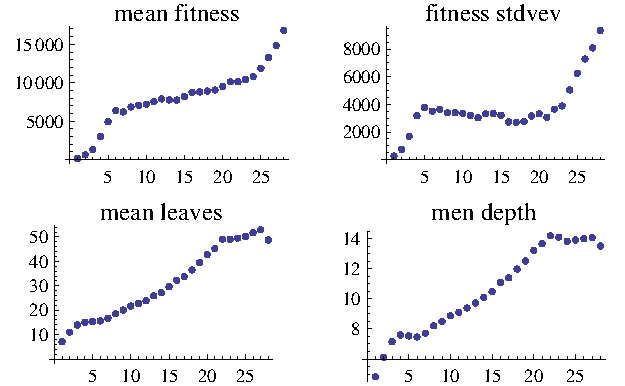
\includegraphics[width=10.0cm]{pr_expr1_run1.pdf}
\caption{output del comando TrendPlot eseguito da PR[]} 
\label{figure:prexpr1}
\end{center}
\end{figure}


con questa configurazione un individui in grado di formare la TargetWord prende 9000 punti di fitness.
infatti dai dati raccolti notiamo che la popolazione di individui giusti cresce fortemente dopo la generazione numero 3.
per vedere meglio questo trend bastera' dare il comando:
\begin{lstlisting}
ListPlot[popgiusti[] ]
\end{lstlisting}

\begin{figure}[!h]
\begin{center}
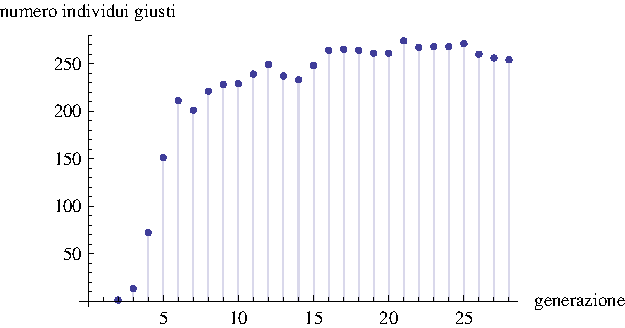
\includegraphics[width=10.0cm]{indgiusti_expr1_run1.pdf}
\caption{output del comando ListPlot[popgiusti[]], la popolazione di individui giusti cresce rapidamente dopo la generazione 4} 
\label{figure:plotpopgiusti1}
\end{center}
\end{figure}

Considerato che la popolazione totale e' di trecento individui, i parametri della fitness considerati sono pienamente soddisfacenti nell'ottica di trovare individui in grado di formare la TargetWord.

Possiamo pero' osservare dalla figura \ref{figure:prexpr1} che la complessita' di questi individui cresce molto rapidamente sia a livello di foglie che di profondita', inoltre gli individui delle generazioni superiore alla 8 hanno tutti un numero di BrokenDu almeno pari a 6 e un numero di step superiore al 60.
\footnote{per orrervare questi aspetti si lanci {\itshape ProfileGeneration[8]} e si osservino i valori della variabile {\itshape valgiusti}. Per approfondire si torni alla sezione \ref{sec:tools} o si veda il file {\itshape tools.m}}

Concludiamo quindi che il package funziona, ma con gli attuali parametri gli individui giusti sono complessi e antieconomici rispetto ai parametri indicati in \ref{item:perf}

\subsubsection{DidSome}
per cercare di ottenere individui piu' semplici ma che ottenessero comunque buoni risultati ho scelto di diminuire fortemente il parametro rlw e aumentare dsw. In questo modo vengono premiati gli individui che alterano la stack.

Inolte per cercare di premiare la semplcita' degli individui e' stata utilizzata la funzione Lol per modulare il punteggio dato da Step e da BrokenDU modificando la fitness nel seguente modo:
\begin{lstlisting}
Fitness[params_]:=Module[{toret},
	(*pesi dei singoli punteggi : *)
	(*i pesi dei punteggi rappresentano l'"ambiente"*)
	rlw	=	100;
	dsw	=	200;
	riw	=	5;
	bdw	=	300;
	stw	=	300;

	mdl = 0;	(*mean step lol*) 
	ddl = 1;	(*delta step lol*) 
	msl = 13;	(*mean broken du lol*) 
	dsl = 5;	(*delta broken du lol*) 

	toret=	params[[1]] rlw + 
			params[[2]] dsw + 
			params[[3]] riw +
			Lol[mdl,ddl,params[[4]]] * 1.0  bdw + 
			Lol[msl,dsl,params[[5]]]  * 1.0 stw ;  
	Return[toret];
];
\end{lstlisting}

cosi' facendo gli individui con BrokenDu pari a zero prenderanno 300 punti e via a scalare con la crescita dei BrokenDU, analogamente piu' gli individui avranno un numero di step pari a 13 piu' potranno ricevere un punteggio aggiuntivo di 300 in base agli step fatti.

Dalle simulazioni fatte, osservando le stack elaborate dagli individui
\footnote{la variabile {\itshape stackdisth} contiene per ogni nerazione il tipo di stack formata e il numero di stack formate},
la tendenza generale e' di svuotare le stack e non di riempirle. 
Inoltre non sono stati trovati individui in grado di ricostruire la Stack, questo vuol dire che il premio dato da didsome e' troppo alto per gli scopi richiesti. Per quanto riguarda la semplicita' degli individui sono stati individuati dei trend di crescita delle foglie e della profondita' simili a figura \ref{figure:prexpr1}.

Un'altra aspetto che e' venuto a galla e' che con l'aumentare delle dimensioni degli individui il tempo di valutazione riservato ad una generazione cresceva a ritmi impressionanti, creando simulazioni che avrebbero impiegato ore a terminare(consideriamo che la popolazione e' di 300 individui, un numero non grande). Per risolvere questo problema e' stata introdotta la variabile MAXDU che termina la valutazione di un individuo quando i suoi BrokenDU superano il valore di MAXDU.

settando MAXDU a 5 il tempo di runtime e' stato notevolmente ridotto, dopotutto individui con un elevato numero di BrokenDU non sono quelli che stiamo cercando.


\subsection{Mimare l'individuo perfetto}
il Package si e' rivelato efficiente nella creazione di individui in grado di creare la TargetWord, ma non di crearne di abbastanza semplici. Si e' quindi scelto di cercare i parametri in grado di mimare le caratteristiche elencate a pag \pageref{item:perf}.

Quello che e' emerso e' che modificare i pesi di bdw e stw non si e' rivelato sufficienete. Infatti sia con parametri come:
\begin{lstlisting}
	rlw	=	50;
	dsw	=	1;
	riw	=	5;
	bdw	=	500;
	stw	=	500;
\end{lstlisting}

che con parametri come
\begin{lstlisting}
	rlw	=	50;
	dsw	=	1;
	riw	=	5;
	bdw	=	500;
	stw	=	1000;
\end{lstlisting}

non si riusciva ad arrestare la crescita delle foglie e della profondita' degli individui per almeno un numero non trascurabile di generazioni.

I parametri che si sono stati decisivi invece sono quelli della funzione Lol.
La funzione Lol che modulava il premio dato agli step ha dato i migliori risultati con una media di 13 step (quelli dell'individuo perfetto) e una sigma di 5.
Provare a stringere la gaussiana a 2 non ha dato risultati soddisfacenti.
Il maggiore impatto l'ha avuto la funzione Lol che modulava il premio dei BrokenDU.

Centrando la gaussiana su 0 e settando la sigma a 3 produceva risultati disastrosi con crescita di complessita' superiore alle precedenti, mentre inpostandola a 2 sono apparsi i primi risultati sperati:

la media delle foglie degli individui restava pari a 9per una decina di generazioni, mentre la profondita' a 5. Dei valori fortemente vicini a quelli cercati.

\lstset{caption=parametri usati per mimare le caratteristiche dell'individuo perfetto,label=source:mim}
\begin{lstlisting}
	rlw	=	50;
	dsw	=	1;
	riw	=	5;
	bdw	=	500;
	stw	=	1000;

	mdl = 0;	(*mean step lol*) 
	ddl = 2;	(*delta step lol*) 
	msl = 13;	(*mean broken du lol*) 
	dsl = 5;	(*delta broken du lol*) 
\end{lstlisting}
\lstset{caption=,label=}

\begin{figure}[!h]
\begin{center}
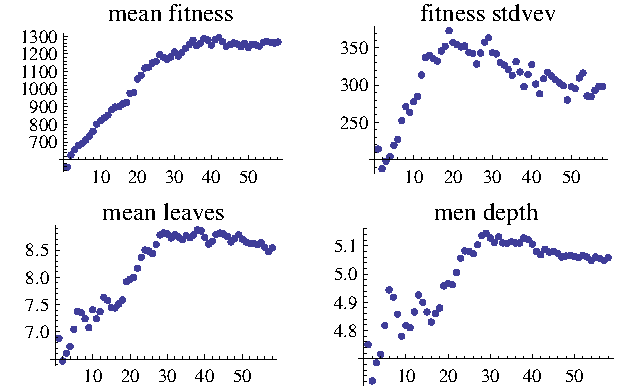
\includegraphics[width=10.0cm]{expr5_run4.pdf}
\caption{risultati ottenuti cercando di mimare l'individuo perfetto con una popolazione di 300 individui. Foglie medie circa 9 e profondita' media circa 5} 
\label{figure:expr5run4}
\end{center}
\end{figure}

Ripetendo le simulazioni con i medesimi parametri i risultati non erano costanti. Su cinque simulazioni effettuate solo due producevano i risultati cercati.
Credendo che questo effetto fosse dovuto ad una mancanza di varieta' del genoma della popolazione ho aumentato il numero degli individui da 300 a 1000 riuscendo finalmente a stabilizzare i risultati. Ognuna delle 5 simulazioni ha dato risultati simili al seguente.

\begin{figure}[!h]
\begin{center}
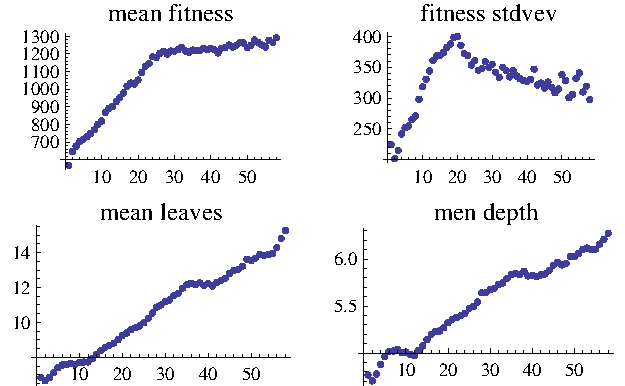
\includegraphics[width=12.0cm]{expr5_run6.pdf}
\caption{risultati ottenuti con una popolazione di 1000 individui e stessi parametri del listato \ref{source:mim}} 
\label{figure:expr5run6}
\end{center}
\end{figure}

nonostante la crescita sia maggiore rispetto a quella in figura \ref{figure:expr5run4} possiamo vedere che le foglie medie sono costanti tra la generazione 35 e la generazione 43.
Questo accade quando la fitness si stabilizza e contemporaneamente la sua deviazione standard diminuisce sensibilmente. Cioe' sempre piu' individui hanno una fitness simile.

Superata la generazione 40 questo la complessita' aumenta velocemente. Chiaramente questa tendenza non puo' essere evitata perche' la complessita' degli individui tendera' a crescere sempre di piu' con l'aumentare delle generazioni perche' il crossover non conserva la lunghezza degli individui. Si ricordi che la fitness non analizza nessuna caratteristica morfologica degli individui ma solo caratteristiche comportamentali. A mano a mano che i crossover aumentano nascono individui con strutture ridondanti che non implicano ne spostamenti di lettere (aumento degli step), ne BrokenDU frequenti (proliferazione di funzioni logiche e di lettura). Per questi motivi ritengo soddisfacente che la media delle foglie si stabilizzi anche solo per un numero di generazioni limitato. Soprattutto il fatto che questo avvenga quando la std della fitness diminuisce, sta ad indicare che nonostante la fitness sia gia' stabile da qualche generazione non ha ancora uniformato la popolazione su una caratteristica preponderante, quando questa uniformazione avviene il numero di foglie si stabilizza.

\subsection{ricerca della perfezione}
A questo punto non resta che trovare l'individuo perfetto. La linea guida da seguire e' di non perdere i caratteri morfologici ottenuti nella sezione precedente e di aumentare la capacita' di creare delle stack corrette.
\subsubsection{primi tentativi, primi fallimenti}
la prima cosa fatta' e' stata chiaramente la piu' intuitiva: lasciare tutti i parametri invariati tranne rlw, facendola aumentare.
intuitivamente pero' rlw non deve amumentare troppo se no la selezione morfologica va a perdersi.

Come primo valore rlw viene settato a 100, questo comporta un punteggio di 900 punti per una stack corretta.
Dai risultati appare che le caratteristiche morfologiche si conservano ma nessun individuo giusto si palesa.

Cercando di movimentare un po' l'azione degli individui amumento il parametro dsw da 1 a 10.
Questo aumenta di gran lunga il numero di individui giusti, ma appaiono essere tremendamente antiestetici e poco funzionali (minimo 6 BrokenDU e 30 step).

Aumentando ancora dsw da 10 a 20 le stack si ritrovano tutte vuote e nessun individuo giusto appare.
lo stesso vale per valori di dsw pari a 50. insomma nonostante il premio per ogni lettera giusta sia di 250 le stack continuano a essere svuotate e non ririempite.

Decido quindi di portare dsw a 1 e di tornare alla configurazione del listato \ref{source:mim} , incrementando rlw fino a 250.
La popolazione di individui giusti tende ad aumentare ma comunque a discapito della semplicita', abbassare rlw a 200 invece non produceva alcun individuo giusto.
Insomma data la configurazione del listato \ref{source:mim} rlw= 250 e' una sorta di soglia di ativazione per la produzione di individui giusti ma tende ad non conservare le caratteristiche di semplicita' degli individui.

\subsubsection{selezione aggressiva}
a questo punto, non potendo piu' agire sui parametri senza perdere in semplicita' ho adottato una tecnica piu' selettiva:
assegnare fitness nulla ad individui con step troppo alti e BrokenDu maggiori di MAXDU.
\footnote{la variabile MAXDU e' gia' stata assegnata per ridurre i tempi di valutazione ma nessn parametro della fitness dipendeva direttamente da lei}

E' stata quindi introdotta la variabile MAXSTEP che segna il mitite di step massimi, sopra questo limite l'individuo viene soppresso, a prescindera delle altre votazioni.
La fitness e' stata quindi modificata come segue:
\begin{lstlisting}
Fitness[params_]:=Module[{toret},

	(*pesi dei singoli punteggi : *)
	(*i pesi dei punteggi rappresentano l'"ambiente"*)
	rlw	=	250;
	dsw	=	1;
	riw	=	5;
	bdw	=	500;
	stw	=	1000;

	mdl = 0;	(*mean step lol*) 
	ddl = 2;	(*delta step lol*) 
	msl = 13;	(*mean broken du lol*) 
	dsl = 5;	(*delta broken du lol*) 

	MAXSTEP = 30;
	(*penalizza fortemente i programmi troppo lunghi*) 
	If[	params[[4]] > MAXDU || params[[5]] >= MAXSTEP,
		toret=	0	,
		toret=	params[[1]] rlw + 
				params[[2]] dsw + 
				params[[3]] riw +
				Lol[mdl,ddl,params[[4]]] * 1.0  bdw + 
				Lol[msl,dsl,params[[5]]]  * 1.0 stw ;  
	];
	Return[toret];
];
\end{lstlisting}

quello che mi aspettavo originariamente con questo approccio era di ottenere individui piu' semplici per piu' generazioni possibili, in modo da contrastare la complessita' crescente, dando la possibilita' di emergere agli individui particolarmente attivi nelle prime fasi.

Infatti settando MAXSTEP=20 sia le foglie che la profondita' resta uguale a quella iniziale per le prime 20 generazioni(si veda figura \ref{figure:expr9run1}), ma gli individui in grado di formare la TargetWord non sono piu' di due per generazione.

Settando MAXSTEP=40 la crescita della complessita' comincia quasi subito.

Molto aristotelicamente assegnando a MAXSTEP il valore di trenta al primo tentativo non solo appaiono molti individui giusti, ma addirittura una popolazione non trascurabile di individui perfetti.

I sisultati della simulazione sono i seguenti:

\begin{lstlisting}
popolazione totale:
1000
popolazione di individui perfetti:
{{20, 1}, {21, 1}, {22, 2}, {23, 3}, {24, 5}, {25, 7}, {26, 8}, {27, 7}, 
 {28, 5}, {29, 7}, {30, 9}, {31, 5}, {32, 4}, {33, 4}, {34, 5}, {35, 2}, 
 {36, 4}, {37, 3}, {38, 4}, {39, 5}, {40, 2}, {42, 2}, {43, 4}, {44, 3}, 
 {45, 4}, {46, 4}, {47, 6}, {48, 5}, {49, 4}, {50, 11}, {51, 6}, {52, 6}, 
 {53, 3}, {54, 4}, {55, 3}, {56, 1}, {57, 1}, {58, 1}, {59, 1}}
popolazione di elementi giusti:
{{2, 1}, {10, 1}, {11, 1}, {12, 3}, {13, 9}, {14, 11}, {15, 19}, {16, 35}, 
 {17, 67}, {18, 115}, {19, 179}, {20, 237}, {21, 293}, {22, 413}, {23, 493}, 
 {24, 566}, {25, 572}, {26, 607}, {27, 590}, {28, 616}, {29, 644}, {30, 664}, 
 {31, 651}, {32, 667}, {33, 647}, {34, 662}, {35, 648}, {36, 701}, {37, 710}, 
 {38, 700}, {39, 707}, {40, 700}, {41, 673}, {42, 689}, {43, 721}, {44, 719}, 
 {45, 747}, {46, 715}, {47, 715}, {48, 732}, {49, 774}, {50, 766}, {51, 763}, 
 {52, 754}, {53, 776}, {54, 783}, {55, 766}, {56, 796}, {57, 823}, {58, 808}}
parametri:
{rlw,dsw,riw,bdw,stw,msl,dsl,mdl,ddl}
{250, 1, 5, 500, 1000, 0, 2, 13, 5}
numero runs:
60
MAXDU:
5
MAXSTEP:
30

\end{lstlisting}

\begin{figure}[!h]
\begin{center}
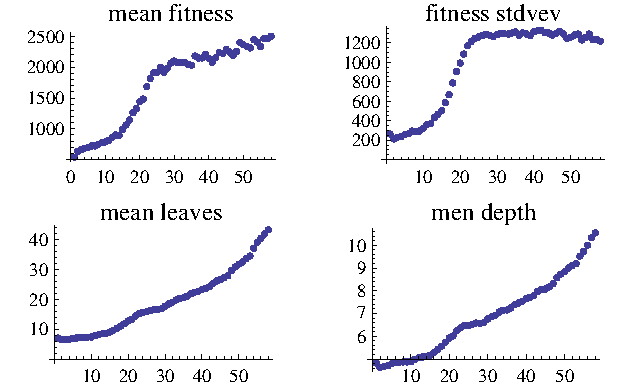
\includegraphics[width=12.0cm]{expr10_run1.pdf}
\caption{trend della simulazione in cui sono apparsi degli individui perfetti.} 
\label{figure:expr10run1}
\end{center}
\end{figure}

con il seguente comando possiamo plottare la distribuzione degli individui perfetti per generazione
\begin{lstlisting}
ListPlot[perfetti[]]
\end{lstlisting}

\begin{figure}[!h]
\begin{center}
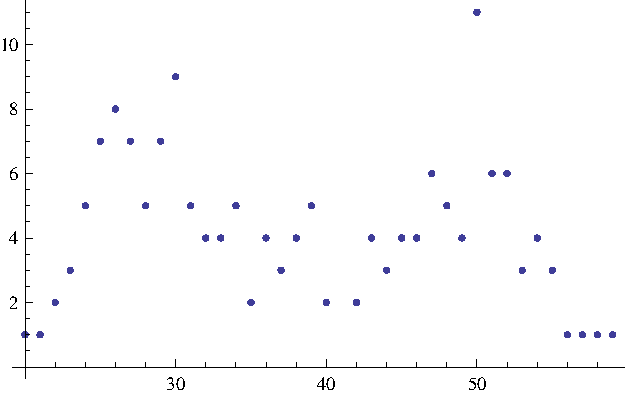
\includegraphics[width=12.0cm]{perfpop.pdf}
\caption{andamento del numero di individui perfetti in funzione della generazione} 
\label{figure:perfdist}
\end{center}
\end{figure}


infine per comparare le popolazioni di individui perfetti con quella di individui giusti si puo' dare semplicemente il comando:
\begin{lstlisting}
ListPlot[{popgiusti[],perfetti[]}]
\end{lstlisting}

\begin{figure}[!h]
\begin{center}
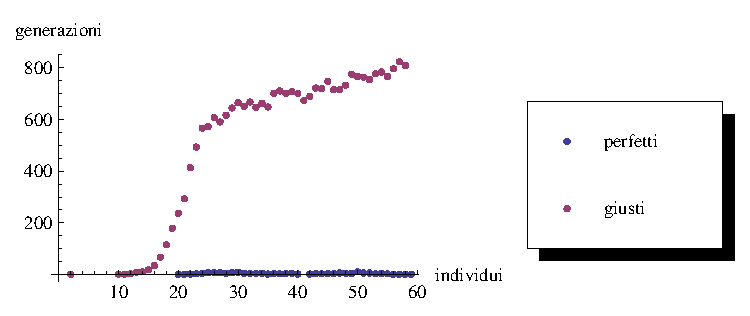
\includegraphics[width=12.0cm]{perfcomp.pdf}
\caption{comparazione del numero di individui perfetti vs numero di individui giusti per generazione} 
\label{figure:perfcomp}
\end{center}
\end{figure}



quello che appare lampante dalla figura \ref{figure:perfcomp} e' che quando esplode la popolazione di individui giusti appaiono anche degli individui perfetti ma che non sono predominanti.
E' difficile anche capire che relazione ci sia tra popolazione di individui giusti e popolazione di individui perfetti guardando la figura \ref{figure:perfdist}, ma il solo fatto che la popolazione di individui perfetti non si estingua e' una soddisfazione notevole.

Possiamo dare una prima interpretazione pensando che quando gli individui perfetti appaiono vengono premiati e tramite CrossOver vengono incapsulati in altri individui piu' complessi, ma che guadagnano in efficienza, facendo esplodere la popolazione di individui giusti.

Purtroppo le simulazioni con questi parametri non danno sempre i risultati sperati, su 11 simulazioni solo 3 hanno avuto risultati simili a questa. In tutti i casi rimanenti la popolazione di individui giusti non esplode affatto. Questo porta dei punti a favore alla spiegazione precedente, senza individui perfetti non c'e' un avanzamento collettivo della popolazione.

\begin{figure}
\begin{center}
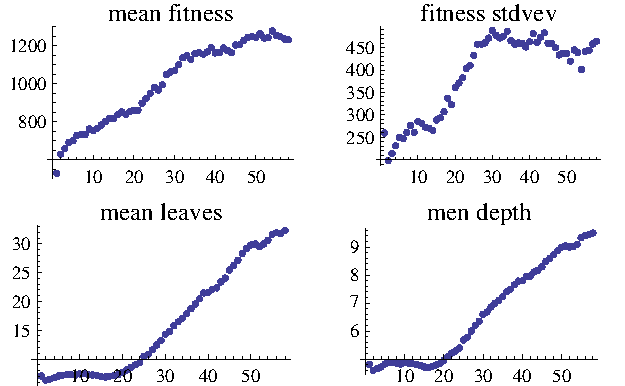
\includegraphics[width=8.0cm]{expr9_run1.pdf}
\caption{con MAXSTEP=20 la complessita' degli individui resta costante per le prime 20 generazioni} 
\label{figure:expr9run1}
\end{center}
\end{figure}


%%%%%%%%%%%%%%%%%%%%%%%%%%%%%%%%%%%%%%%%%%%%%%%%%%%%%%%%%%%%%%%%%%%%%%%%%%%%%%%%%%%%%%%%%%%%%%%%%%%%%%%%%%%%%%%%%%%%%%%%%%%%
%%%%%%%%%%%%%%%%%%%%%%%%%%%%%%%%%%%%%%%%%%%%%%%%%%%%%%%%%%%%%%%%%%%%%%%%%%%%%%%%%%%%%%%%%%%%%%%%%%%%%%%%%%%%%%%%%%%%%%%%%%%%
%%%%%%%%%%%%%%%%%%%%%%%%%%%%%%%%%%%%%%%%%%%%%%%%%%%%%%%%%%%%%%%%%%%%%%%%%%%%%%%%%%%%%%%%%%%%%%%%%%%%%%%%%%%%%%%%%%%%%%%%%%%%

\section{Ottimizzazione e Possibili Sviluppi}
\label{sec:opti}
Per quanto riguarda l'ottimizzazione questo programma e' molto e adatto alla parallelizzazione. La parte computazionalmente piu' impegnativa e' la valutazione degli individui che e' un operazione indipendente e relativamente facile da implementare, tutti ingredienti adatti per la parallelizzazione magari su gpu(memoria permettendo). Lo stesso ragionamento vale per la fitness, il CrossOver, il Profiling e la Mutazione. Sono tutte operazioni indipendenti e relativamente facili.

Per quanto riguarda i miglioramenti del mio codice bisogna pensare a scrivere una funzione di Mutazione che garantisca la correttezza sintattica, cosa che non ho fatto per mancanza di tempo. Inolte bisognerebbe implementare una versione di HAC che risolva il problema DUT DUW sulla posizione del ramo e non passando una Head ad hoc come ho fatto (non avevo ancora acquisito buone conoscenze del comando Position quando ho implementato {\itshape firstgen.m }).

Infine si potrebbe dedicare piu' tempo alla ricerca della giusta combinazione di parametri e condizioni per creare una popolazione di elementi perfetti nelle prime generazioni con costanza. Confido pero' nella struttura del mio Package e ritengo sia primariamente una questione di tempo.

Infine sarebbe bello testare l'algoritmo in casi in cui l'individuo perfetto scritto nella sezione \ref{sec:exp}, non sia il migliore. Per esempio nel caso in cui la DefaultStack presentasse gia' delle lettere in posizioni corrette, per le quali sarebbe inutile riposizionarle a terra.

\section{Conclusioni personali}
Per quanto questo esercizio sia astratto mi ha forzato a comprendere il cuore del linguaggio che utilizza {\itshape Mathematica}: la struttura delle espressioni. Ritengo che avere una buona conoscenza di base di un linguaggio cosi' astratto sia decisamente una cosa costruttiva ed educativa.

Essendo abituato al massimo a livelli procedurali od ObjectOriented ho sicuramente fatto fatica ad abituarmi all'inizio, ma dopo le difficolta' iniziali l'apprendimento si e' rivelato veloce e appagante. Il maggior sforzo e' stato nell'acquisire una mentalita' molto piu' flessibile e non piu' incentrata sui tipi di dato ma sulle espressioni ed i pattern.
L'aver potuto scrivere una funzione concettualmente complessa come HAC in tre righe di codice rende onore a questo linguaggio e alla sua praticita'.

Dal punto di vista delle prestazioni sono rimasto piacevolmente colpito dall'uso modico dell memoria che e' stato fatto durante le simulazioni, anche con popolazioni di 5000 individui.
E' chiaro che questa flessibilita' vada a discapito di un utilizzo della CPU molto elevato. Dati i tempi di runtime di questo Package bisogna seriamente tenere in considerazione che il tempo risparmiato a scrivere il codice e' pienamente sufficiente per compensare il tempo di computazione.

Un altro risparmio di tempo notevole e' dovuto alla flessibilita' del linguaggio rispetto al C++ per esempio. Con i linguaggi OO a basso livello sarebbe stato necessario un lungo periodo di design e la scrittura ``a braccio'' del codice andrebbe ridotta al minimo. Con {\itshape Mathematica} problemi complessi possono essere risolti in una giornata e la produttivita' dello sviluppatore e' decisamente superiore alla media.

Sinceramente sarei curioso di vedere come si comporta {\itshape Mathematica} con progetti che hanno una mole molto maggiore sia a livello di moduli che di codice.

Una cosa a cui non sono pero' riuscito ad abituarmi e' la mancanza di  un bebugger che permetta di eseguire riga per riga il codice a livello di Kernell, secondo me una qualita' insostituibile che deve avere un linguaggio, per quanto sia scritto per ridurre al minimo il Debug.


%%%%%%%%%%%%%%%%%%%%%%%%%%%%%%%%%%%%%%%%%%%%%%%%%%%%%%%%%%%%%%%%%%%%%%%%%%%%%%%%%%%%%%%%%%%%%%%%%%%%%%%%%%%%%%%%%%%%%%%%%%%%
%%%%%%%%%%%%%%%%%%%%%%%%%%%%%%%%%%%%%%%%%%%%%%%%%%%%%%%%%%%%%%%%%%%%%%%%%%%%%%%%%%%%%%%%%%%%%%%%%%%%%%%%%%%%%%%%%%%%%%%%%%%%
%%%%%%%%%%%%%%%%%%%%%%%%%%%%%%%%%%%%%%%%%%%%%%%%%%%%%%%%%%%%%%%%%%%%%%%%%%%%%%%%%%%%%%%%%%%%%%%%%%%%%%%%%%%%%%%%%%%%%%%%%%%%

\section{Sorgenti}
\label{sec:source}
\subsection{moves.m}
\lstinputlisting{moves.m}
\subsection{firstgen.m}
\lstinputlisting{firstgen.m}
\subsection{crossover.m}
\lstinputlisting{crossover.m}
\subsection{fitness.m}
\lstinputlisting{fitness.m}
\subsection{tools.m}
\lstinputlisting{tools.m}


%%%%%%%%%%%%%%%%%%%%%%%%%%%%%%%%%%%%%%%%%%%%%%%%%%%%%%%%%%%%%%%%%%%%%%%%%%%%%%%%%%%%%%%%%%%%%%%%%%%%%%%%%%%%%%%%%%%%%%%%%%%%
%%%%%%%%%%%%%%%%%%%%%%%%%%%%%%%%%%%%%%%%%%%%%%%%%%%%%%%%%%%%%%%%%%%%%%%%%%%%%%%%%%%%%%%%%%%%%%%%%%%%%%%%%%%%%%%%%%%%%%%%%%%%
%%%%%%%%%%%%%%%%%%%%%%%%%%%%%%%%%%%%%%%%%%%%%%%%%%%%%%%%%%%%%%%%%%%%%%%%%%%%%%%%%%%%%%%%%%%%%%%%%%%%%%%%%%%%%%%%%%%%%%%%%%%%



\begin{thebibliography}{1}
 
 \providebibliographyfont{name}{}%
  \providebibliographyfont{lastname}{}%
  \providebibliographyfont{title}{\emph}%
  \providebibliographyfont{jtitle}{\btxtitlefont}%
  \providebibliographyfont{etal}{\emph}%
  \providebibliographyfont{journal}{}%
  \providebibliographyfont{volume}{}%
  \providebibliographyfont{ISBN}{\MakeUppercase}%
  \providebibliographyfont{ISSN}{\MakeUppercase}%
  \providebibliographyfont{url}{\url}%
  \providebibliographyfont{numeral}{}%
  \expandafter\btxselectlanguage\expandafter {\btxfallbacklanguage}

\expandafter\btxselectlanguage\expandafter {\btxfallbacklanguage}


\bibitem {mathematica8}
\btxnamefont {\btxlastnamefont {{Wolfram Research, Inc.}}}\btxauthorcolon\
  \btxtitlefont {\btxifchangecase {{Mathematica Edition: Version
  8.0}}{{Mathematica Edition: Version 8.0}}}, {2010}.

\bibitem{mitchell}
\btxnamefont {\btxlastnamefont {{Melanie Mitchell}}}\btxauthorcolon\
  \btxtitlefont {\btxifchangecase {{An Introduction to Genetic Algorithms
    }}{{MIT Press: Fith printing}}}, {1999}.

\end{thebibliography}

\end{document}
